% Guangdong science 2011 pyramid schematic.
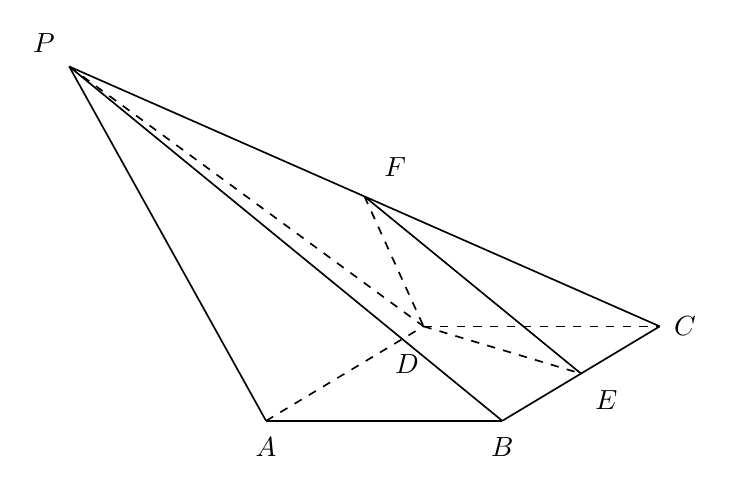
\begin{tikzpicture}[x=1cm,y=1cm,font=\normalsize,
  geometry edge/.style={draw=black,solid,line width=.6pt},
  geometry hidden/.style={draw=black,dashed,line width=.6pt},
  geometry label/.style={font=\normalsize,inner sep=2pt,fill=none}]
\coordinate (P) at (-1.0,4.5);
\coordinate (A) at (1.5,0.0);
\coordinate (B) at (4.5,0.0);
\coordinate (D) at (3.5,1.2);
\coordinate (C) at (6.5,1.2);
\coordinate (E) at (5.5,0.6);
\coordinate (F) at (2.75,2.85);
\draw[geometry hidden] (P)--(D);
\draw[geometry hidden] (A)--(D);
\draw[geometry hidden] (D)--(C);
\draw[geometry hidden] (D)--(E);
\draw[geometry hidden] (F)--(D);
\draw[geometry edge] (A)--(B);
\draw[geometry edge] (B)--(E)--(C);

\draw[geometry edge] (P)--(A);
\draw[geometry edge] (P)--(B);
\draw[geometry edge] (P)--(F)--(C);
\draw[geometry edge] (F)--(E);
\node[geometry label,above left,xshift=-3pt,yshift=3pt] at (P) {$P$};
\node[geometry label,below,yshift=-4pt] at (A) {$A$};
\node[geometry label,below,yshift=-4pt] at (B) {$B$};
\node[geometry label,below,yshift=-2pt,xshift=-6.00bp,yshift=-6.00bp] at (D) {$D$};
\node[geometry label,right,xshift=3pt] at (C) {$C$};
\node[geometry label,below right,xshift=3pt,yshift=-4pt] at (E) {$E$};
\node[geometry label,above right,xshift=5pt,yshift=5pt] at (F) {$F$};
\end{tikzpicture}